\documentclass[a4paper, 11pt]{article} % Font size (can be 10pt, 11pt or 12pt) and paper size (remove a4paper for US letter paper)

\usepackage[T1]{fontenc}
\usepackage[utf8]{inputenc}
\usepackage[ngerman]{babel}
\usepackage{lmodern}

\usepackage[protrusion=true,expansion=true]{microtype} % Better typography
\usepackage{graphicx} % Required for including pictures
\usepackage{wrapfig} % Allows in-line images
\usepackage{amssymb,amsmath}
\usepackage{subfigure}
\usepackage{cite}
\usepackage{mathpazo} % Use the Palatino font
\linespread{1.05} % Change line spacing here, Palatino benefits from a slight increase by default

\usepackage{tikz-uml}
%\usepackage{tikz}
%\usepackage{ifthen}
%\usepackage{xstring}
%\usepackage{calc}
%\usepackage{pgfopts}

\usepackage{listings}

%\setlength\parindent{0pt}%Festlegen des Absatzeinzuges
%\setlength\mathindent{0pt}%Festlegen des Einzuges für abgesetzte Formeln

\setlength{\parindent}{0pt} 

\makeatletter
\renewcommand\@biblabel[1]{\textbf{#1.}} % Change the square brackets for each bibliography item from '[1]' to '1.'
\renewcommand{\@listI}{\itemsep=0pt} % Reduce the space between items in the itemize and enumerate environments and the bibliography

\renewcommand{\maketitle}{ % Customize the title - do not edit title and author name here, see the TITLE block below
\begin{flushright} % Right align
{\LARGE\@title} % Increase the font size of the title

\vspace{50pt} % Some vertical space between the title and author name

{\large\@author} % Author name
\\\@date % Date

\vspace{40pt} % Some vertical space between the author block and abstract
\end{flushright}
}

\title{\textbf{Dokumentation gMix-Simulator GUI}\\ % Title
Benutzer- / Entwicklerhandbuch} % Subtitle

\author{\textsc{Beifuß A. ; Langnickel J. ; Lohmueller J. C. ; Weinschenk M.} % Author
\\{\textit{Universität Hamburg - MIN Falkultaet - Informatik - SVS}}} % Institution

\date{\today} % Date

\begin{document}

\maketitle % Print the title section

%\renewcommand{\abstractname}{Summary} % Uncomment to\texttt{} change the name of the abstract to something else
 
% \begin{abstract}

% \end{abstract}

\tableofcontents

% \hspace*{3,6mm}\textit{Keywords:} lorem , ipsum , dolor , sit amet , lectus % Keywords

\vspace{30pt} % Some vertical space between the abstract and first section

\section{Einleitung} % (fold)
\label{sec:einleitung}

\subsection{gMix (Todo Malte)} % (fold)
\label{sub:gmix}
Dieser Abschnitt behandelt das Thema Mixe und motiviert die Entwicklung des gMix-Simulators. \cite{Cha81}
% subsection gmix (end)

\subsection{Ziele der GUI (Todo Malte)} % (fold)ssu
\label{sub:ziele_der_gui}
In diesem Abschnitt werden die unterschiedlichen Benutzergruppen vorgestellt, für die GUI gedacht ist. Es wird analysiert, welche Anforderungen und Bedürfnisse die jeweiligen Anwendergruppen haben. Entlang der gewonnenen Erkenntnissen soll dann die GUI entwickelt werden, so dass nach Möglichkeit die Anforderungen aller Gruppen zufriedengestellt werden können.
% subsection ziele_der_gui (end)

\subsection{XML vs. Annotations} % (fold)
\label{sub:xml}
In diesem Abschnitt werden wir kurz motivieren, warum wir uns bei der Entwicklung der gMix GUI für die Verwendung Annotations und nicht für die Verwendung XML entschieden haben.\\

\textbf{Flexibilität / Erweiterbarkeit:}\\
Ein sehr wichtiger Aspekt ist, dass das von uns angestrebte Annotations-System sehr einfach erweiterbar sein soll. Da der \emph{gMix-Simulator} Plugin-basiert ist, kann es zu einem späteren Zeitpunkt (nach Projektende) notwendig sein, dass \emph{Properites} oder \emph{Plugins} beispielsweise um neue Eigenschaften erweitert werden sollen. Während im Falle von XML ggf. das Schema angepasst werden und muss komplexere Eingriffe in das Parsing notwendig sein können, ist der Aufwand bei der Verwendung von Annotations sehr gering. Hier genügt es die jeweiligen Annotations (beispielsweise \emph{IntSimulationProperty}), um die notwendigen Felder zu erweitern. Die zugehörigen POJOs (beispielsweise \emph{IntProp}), welche später die Informationen aus den Annotationen enthalten, müssen lediglich um \emph{Getter} und \emph{Setter} erweitert werden. Die notwendigen Änderungen am Annotations-Parser (in der Klasse \emph{SimPropRegistry}) sind ebenfalls sehr einfach und beschränken sich auf das Auslesen der Annotation und das Aufrufen von \emph{Settern}.\\

\textbf{Dezentralisierung:}\\
Im Gegensatz zu XML werden Annotationen direkt in den Plugin-Code eingebettet. Dieses bringt gleich zwei Vorteile mit sich. Zum einen werden dadurch zentrale Dateien vermieden, wodurch eine sehr lose Kopplung ermöglicht wird, wie es bei Plugin-Systemen wünschenswert ist --- Versionskonflikte von zentralen Dateien werden so vermieden. Dieses ist bei Plugin-System sehr wichtig. Allerdings wäre eine lose Kopplung auch noch mit XML möglich, würde jedoch unweigerlich in einer Unmenge an XML-Dateien enden, sofern jedes Plugin eine eigene XML Datei erhält. Der zweite Vorteil ist, dass ein Pluginentwickler die Festlegung der Eigenschaften von Properties und Plugins genau dort vornimmt, wo diese auch logisch gesehen hingehören, nämlich direkt an den Properties und den Plugins selbst. Dieses ist gerade bei der Entwicklung neuer Plugins von Vorteil, da nicht permanent zwischen mehreren Dateien (Java Code und XML Datei) hin und her gesprungen werden muss. Bei der Erweiterung von existierendem Code kann dieses jedoch auch nachteilig sein, da der Entwickler ggf. erst nach der relevanten Stelle im Code suchen muss und nicht wie bei XML alle Informationen in einer bekannten Datei vorliegen hat.\\

Ein dritter Aspekt ist, dass Annotationen ein Teil der Sprache Java sind. Dieses bedeutet für einen Entwickler, dass er bei den Programmieraufgaben mehr Unterstützung durch die IDE bekommt, als es bei XML möglich ist. So wird er bei der Erweiterung von Annotationen beispielsweise frühzeitig auf syntaktische und semantische Fehleraufmerksam gemacht. Bei der Verwendung von XML ist dieses nicht gegeben, da zwischen der XML-Datei und Java-Code kein syntaktischer Zusammenhang besteht. Die Erkennung von semantischen Fehlern ist bei XML dadurch eingeschränkt, da XML code keine Typen wie kennt und somit nicht erkennen kann, ob eine Eingabe valide ist.\\

Für den Anwender der GUI ist die Wahl zwischen Annotationen und XML irrelevant, da dieses aus seiner Sicht transparent ist. Der Pluginentwickler profitiert jedoch im Normalfall ein klein wenig mehr von dem Einsatz von Annotationen. Aus diesem Grund haben wir uns entschieden ein neues Framework (basierend auf Annotationen) zu entwickeln und nicht auf ein (aus einem früheren Projekt verfügbaren) XML basierendes Framework zurückzugreifen.

% subsection xml (end)

% section einleitung (end)

\newpage
\subsection{Annotations} % (fold)
\label{sub:annotations}
Dieser Abschnitt beschreibt die unterschiedlichen Annotation-Typen, welche unsere GUI verwendet. Insgesamt sind es drei unterschiedliche Typen von Annoations, die in der GUI zum Einsatz kommen. Es werden nun die Annotations-Typen motiviert, ihre Unterschiede erläutert. Weiterhin wird ausführlich auf die einzelnen Felder der Annotationen eingegangen.\\

Um den Leser mit der von uns verwendeten Bezeichnungen in Bezug auf die GUI-Elemente bekannt zu machen, dient die nachfolgende Abbildung \ref{fig:guielements} . 

\begin{figure}[!htp]

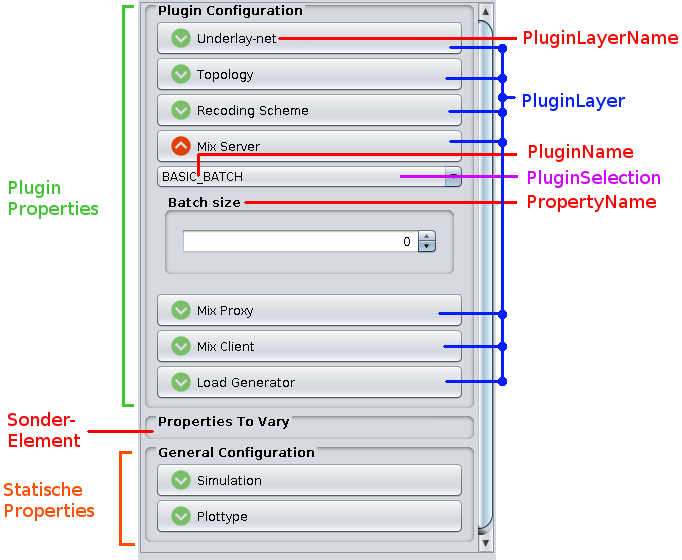
\includegraphics[scale=0.56]{img/configtool_edit.png}
% subsection annotations (end)

\caption{Ausschnitt des 'Config Tools'}
\label{fig:guielements}
\end{figure}

Bevor es die gMix GUI gab wurde die Konfiguration des Simulators in einer Textdatei (EDF - Experiment Definition File) vorgenommen. Ein Auszug aus einer solchen Konfigurationsdatei ist in Listing \ref{lst:edf} dargestellt.

\newpage

\begin{lstlisting}[caption={Auszug aus einer Simulator Konfiguration},label=lst:edf,frame=lrtb]
#-OUTPUT_STRATEGY--OR--FLUSHING_ALGORITHM----------
# ...
# Some possible values: NO_DELAY, ... 
# BATCH_WITH_TIMEOUT, BINOMIAL_POOL, ... 
# COTTRELL_TIMED_POOL, DISTINCT_USER_BATCH, ... 
# DLPA_HEURISTIC_2, LOSSY_SYNCHRONOUS_BATCH, ...
# THRESHOLD_AND_TIMED_BATCH, THRESHOLD_OR_TIMED_BATCH 
# TIMED_BATCH, TIMED_DYNAMIC_POOL
#	
OUTPUT_STRATEGY = BASIC_BATCH
...
BASIC_BATCH_BATCH_SIZE = 100
...
\end{lstlisting}

Eine Hauptaufgabe unserer Arbeit bestand nun darin eine geeignete Abbildung zu finden, die es erlaubt die Inhalte der Konfigurationsdatei grafisch darzustellen. Es zeigte sich, dass hierfür eine hierarchische Struktur mit drei Ebenen geeignet ist (vergleiche Abb. \ref{fig:guielements}).

\begin{itemize}
	\item Layer: Die Auswahl des Layers legt fest, welches Plugin als Implementation für einen bestimmten Software-Layer während der Simulation verwendet werden soll. Die einzelnen Layer des gMix Simulators können in Abschnitt \ref{sub:gmix} nachgelesen werden. 
	\item Plugin: Als Plugin wird eine in sich geschlossene Implementation einer bestimmten Funktionalität verstanden. Jeder Layer setzt eine gewisse Schnittstelle (für die auf dem Layer agierenden Plugin) voraus, legt dabei jedoch nicht fest, wie die Implementation selbst auszusehen hat.
	\item Property: Je nach Implementation benötigt ein Plugin Parameter, um gewisse interne Variablen zu konfigurieren. Anzahl, Typ und zulässige Werte dieser Parameter hängen jedoch mit der Implementation des Plugins zusammen und müssen von dem Experimentator festgelegt werden. Zu diesem Zweck muss ein Plugin je Parameter eine Property definieren, die der Experimentator schließlich setzen darf.
\end{itemize} 

Im Listing \ref{lst:edf} ist 'OUTPUT\_STRATEGY' der PluginLayerKey für das Plugin, welches auf der Ebene (Layer) des Mix-Servers (bzw. der Ausgabestrategie - Output Strategy) argiert. In der Experiment-Konfiguration bildet der PluginLayerKey auf ein PluginKey ab (hier 'BASIC\_BATCH') und identifiziert damit das aktive Plugin (hier 'BASIC\_BATCH'). Das Plugin, welches den PluginKey 'BASIC\_BATCH' zugewiesen ist, hat wiederum eine Property, welche durch den PropertyKey 'BASIC\_BATCH\_BATCH\_SIZE' identifiziert wird (Dieses geht nicht aus der EDF hervor, sondern ist im Code des Simulators verankert).\\

Nachdem nun die grundlegenden Terminologien eingeführt wurden, wollen wir die Annotations betrachten, welche den Aufbau der GUI regeln. Wir gehen dabei bottom-up vor, da weniger Informationen vorweggenommen werden müssen und die Argumentation somit für den Leser ein wenig verständlicher sein sollte.

\subsubsection{Property Annotation} % (fold)
\label{ssub:feld_annotation}
Die Property-Anotations sind wohl die wichtigsten und auch komplexesten Annotations, die wir in der GUI verwenden. Diese Annotations werden dazu verwendet um Felder im Quellcode des Simulators und im Quellcode der Plugins zu annotieren. Dabei werden solche Felder annotiert, die tatsächlich Simulation-Properties halten. Diese sind daran zu erkennen, dass ihr Wert über \emph{Simulator.settings.getProperty()} abgefragt wird, um den Simulator oder ein Plugin zu parametrisieren.\\

Alle \emph{Properties} haben eine gewisse Grundmenge an Feldern, die in der folgenden Auflistung erläutert werden. Besonders sei hier die \emph{BoolSimulationProperty} hervorgehoben. Dieses ist die einzige Property-Annotation, die außer dieser Grundmenge keine weiteren Felder besitzt.
\begin{itemize}
	\item \textbf{name:} Es handelt sich um einen String, der den Namen der Property festlegt, wie er in der GUI angezeigt werden soll. Analog zur obigen Grafik entspricht dieses dem \emph{PropertyName}.\\
	\textbf{Default:} keinen (Der Entwickler muss diesen Wert händisch setzen)
	\item \textbf{key:} Ein String der die Property innerhalb der Experiment-Konfiguration eindeutig identifiziert. Analog zum obigen Listing entspricht dieses dem \emph{PropertyKey}).
	\item \textbf{position:} Dieses ist ein Integer (>= 0), der die Position des zugehörigen GUI-Elementes steuert. Je größer der Wert desto weiter unten taucht das GUI-Element der jeweiligen Proerty auf. Sollten zwei Properties eines Plugins hier den selben Wert haben, so wird lexikalisch geordnet.\\
	\textbf{Defalut: 0}\\
	\textbf{Anmerkung: noch nicht vollständig implementiert}
	\item \textbf{tooltip:} Dieses ist ein String, der angezeigt wird, wenn sich die Maus über dem entsprechenden GUI-Element befindet.\\
	\textbf{Default:} leerer String 
	\item \textbf{info:} Ein String der (sofern festgelegt) als Infotext an dem entsprechenden GUI-Element der Property auftaucht.  
	\textbf{Default: leerer String}
	\item \textbf{global:} Ein Boolean über das festgelegt werden kann, dass die Property global (im gesamten PluginLayer angezeigt werden soll).\\
	\textbf{Default:} false
	\item \textbf{inject:} Ein String der es erlaubt Properties an eine beliebige Stelle in der GUI zu injizieren. Dieses ist notwendig, wenn Properties beispielsweise zu einem pseudo Plugin gehören (\emph{'Recoding Scheme'} ist z.B. ein solches pseudo Plugin, das in Wirklichkeit nicht als Plugin existiert sondern viel Mehr direkt im Simulator integriert ist, dem Benutzer jedoch als Plugin dargestellt werden soll). \\
	\textbf{Syntax:} \"{}<LayerPosition>:<LayerKey>,<LayerName> [@<PluginPosition>:<PluginKey>,<PluginName>]\"{}\\
	Wird hier der optionale Plugin-Teil weggelassen, so gibt die Property als Layerweit (global) sichtbar.\\
	\textbf{Default:} leerer String (keine Injection)
	\item \textbf{isStatic:} Ein Boolean das angibt, ob eine Property im Plugin-Abschnitt (\emph{Plugin Configuration}) auftauchen soll oder aber im Abschnitt für statische Properties (\emph{General Configuration}). Dieses Feld wird nur in Kombination mit dem Feld \emph{inject} verwendet. Sinnvoll ist der Einsatz meist dort, wo es sich um Properties handelt, die nicht zu einem Plugin gehören und aus logischer Sicht auch nicht auf einer Pluginschicht liegen.\\
	\textbf{Default:} false (Property wird in der \emph{Plugin Configuration} angezeigt)
	\item \textbf{value\_requirements:} Eine Klasse, welche von der abstrakten Klasse Requirement erbt und in derer für diese Simproperty relevante Werte Anforderungen umgesetzt werden.
	\item \textbf{enable\_requirements:} Eine Klasse, welche von der abstrakten Klasse Requirement erbt und in derer für diese Simproperty relevante Freischalte Anforderungen umgesetzt werden.
\end{itemize}

Die Annotationen für die numerischen \emph{Properties} (\emph{IntSimulationProperty}, \emph{FloatSimulationProperty} und \emph{DoubleSimulationProperty}) haben neben den Standardfeldern noch Felder, welche hauptsächlich die gültigen Wertebereiche betreffen.
\begin{itemize}
	\item \textbf{min:} Ein numerischer Wert (abhängig vom konkreten Typ der Annotation), der den Minimalwert angibt, den die Property annehmen kann. Der angegebene Wert wird von der GUI dazu verwendet um Benutzereingaben auf Gültigkeit zu prüfen.\\
	\textbf{Default:} Integer.MIN\_VALUE bzw. Float|Double.NEGATIVE\_INFINITY
	\item \textbf{max:} Ein numerischer Wert (abhängig vom konkreten Typ der Annotation), der den Maximalwert angibt, den die Property annehmen kann. Der angegebene Wert wird von der GUI dazu verwendet um Benutzereingaben auf Gültigkeit zu prüfen.\\
	\textbf{Default:} Integer|Float|Double.MAX\_VALUE
	\item \textbf{guiElement:} Ein String über den festgelegt werden kann, über was für ein GUI-Element der Wert Property in der GUI konfiguriert werden kann. Aktuell sind für Ganzzahl und Gleitkomma zahlen die beiden Elemente JSpinner (\emph{\"{}spinner\"{}} für Integer, Float und Double) und JSlider (\emph{\"{}slider\"{}} für Integer) implementiert. Beide Elemente verwenden die durch die Felder \emph{min} und \emph{max} festgelegten Grenzen und schützen den Benutzer vor Fehleingaben.\\
	\textbf{Default:} \emph{\"{}spinner\"{}} (JSpinner)
	\item \textbf{stepSize:} Ein numerischer Wert (abhängig vom konkreten Typ der Annotation), der die Schrittweite eines JSpinners angibt. Dieses Feld ist in Kombination mit \emph{guiElement=\"{}spinner\"{}} sinnvoll, um die Schrittweite manuell festzulegen. So ist es bei einigen Properties vlt. besser eine Schrittweite von 0.1 zu haben, während bei anderen Properties vielleicht kleinere Schrittweiten wie 0.001 besser passen.\\
	\textbf{Default:} Integer 1, Gleitkomma 0.001f
	\item \textbf{enableAuto:} Ein Boolean über das festgelegt werden kann, dass die eigentlich numerische Property den String \"{}AUTO\"{} annehmen kann. Der Simulator sieht dieses für einige Properties vor. Im Falle, dass eine numerische Property den Wert \"{}AUTO\"{} hat, wird der tatsächliche Wert automatisch anhand von anderen Properties bestimmt. Wird dieses Feld auf true gesetzt, so gibt es im entsprechenden GUI-Element eine Checkbox, über die der Benutzer festlegen kann, dass die Property automatisch bestimmt werden soll. Für denn Fall, dass  die Checkbox aktiviert ist, wird das eigentliche Eingabeelement (siehe \emph{guiElement}) ausgegraut.\\
	\textbf{Beispiele:} Request und Reply Size in ParetoClient, PoissonClient, RequestReplyClient und SendConstantClient\\
	\textbf{Default:} false (keine Checkbox für \"{}AUTO\"{}) 
	\item \textbf{enableUnlimited:} Ein Boolean über das festgelegt werden kann, dass die eigentlich numerische Property den String \"{}UNLIMMITED\"{} annehmen kann. Dieses funktioniert analog zu \emph{enableAuto}.\\
	\textbf{Beispiel:} DelayBox alle sechs Bandwidth-Properties
	\textbf{Default:} false (keine Checkbox für \"{}UNLIMITED\"{})
\end{itemize}

Die Annotation \emph{StringSimulationProperty} hat ebenfalls zusätzliche Felder.
\begin{itemize}
	\item \textbf{possibleValues:} Ein String über den vordefinierte Werte festgelegt werden können. Die einzelnen Werte werden innerhalb des Strings durch Kommata separiert. Ist dieser String ungleich dem leeren String, so wird die GUI dem Benutzer eine JCombobox zur Manipulation des Property-Wertes anbieten (es sei denn, dass \emph{multiSelection=true} ist, siehe nächstes Feld).\\
	\textbf{Default:} leerer String
	\item \textbf{multiSelection:} Ein Boolean über den festgelegt werden kann, dass eine Mehrfachauswahl der vordefinierten Werte möglich ist. Ist dieses Feld auf true gesetzt und sind mittels \emph{possibleValues} mehrere vordefinierte Werte angegeben, so wird ein, auf einer JList basierendes, GUI-Element erstellt, die eine Mehrfachauswahl erlaubt.\\
	\textbf{Default:} false (Mehrfachauswahl ist deaktiviert) 
	\item \textbf{regex:} Ein String der eine Regex darstellt, die dazu verwendet wird, um Benutzereingaben auf Gültigkeit zu prüfen (kann dann ggf. auch in den ValueRequirements verwendet werden!)
	\textbf{Anmerkung:} noch nicht vollständig implementiert\\
	\textbf{Default:} leerer String
\end{itemize}

% subsubsection feld_annotation (end)

\subsubsection{Plugin Annotation} % (fold)
\label{ssub:plugin_annotation}
Neben den \emph{Property Annotations} gibt es zwei weitere Typen von Annotations. Hierzu gehören unter anderem die \emph{Plugin Annotations}. Die Einführung dieser Annotations erschien uns aus dem Grund sinnvoll, da es für einen Pluginentwickler vorteilhaft ist, wenn dieser Eigenschaften, die logisch gesehen zu einem Plugin gehören, auch direkt am Plugin setzten kann. Beispiele hierfür sind der Pluginname, der in der GUI auftaucht (z.B. ''Basic delay box'') oder aber der Schlüssel, unter dem das Plugin in der Experiment-Konfiguration auftaucht (z.B. ''BASIC\_DELAY\_BOX''). Des weiteren erlaubt eine Annotation auf Pluginebene das pluginweite setzen von Eigenschaften. So kann beispielsweise über eine \emph{Property Annotation} festgelegt werden, dass alle Properties, welche in einem Plugin liegen global sind, wodurch sich der Pluginentwickler ggf. ein wenig Schreibarbeit sparen kann. \emph{Property Annotations} haben folgende Felder:

\begin{itemize}
	\item \textbf{pluginName:} Ein String, der den Namen festlegt, unter dem das Plugin in der GUI auftritt. Entspricht der bereitgestellt String dem leeren String, so wird stattdessen \emph{pluginKey} als angezeigter Name in der GUI verwendet.\\
	\textbf{Default:} Der leere String
	\item \textbf{pluginKey:} Ein String, der dem Namen festlegt, unter dem das Plugin in der Experiment-Konfiguration auftritt. Dieser String muss dabei genau dem String entsprechen, der das Plugin gegenüber dem den \emph{gMix-Simulator} identifiziert (siehe Enums in \emph{evaluation.simulator.pluginRegistry}).
	\item \textbf{pluginLayerKey:} Ein String, der den Layer (also die Kategorie) festlegt, unter dessen Pluginauswahl das Plugin auftauchen soll. Dieses Feld ist dafür gedacht, dass der Entwickler von Hand festlegen kann, in welchem Layer das Plugin aufgelistet wird. Dieses ist notwendig, wenn ein Plugin aus mehreren Klassen besteht die keine gemeinsame Oberklasse haben. Ein Beispiel für die Anwendung dieses Feldes ist in der Klasse \emph{StopAndGoMessage} zu finden. Dort wird mittels dieses Feld mitgeteilt, dass dieses Plugin in den Layer \"{}OUTPUT\_STRATEGY" gehört. Der Layer selbst wird aber durch die \emph{Plugin Superclass Annotation} in \emph{OutputStrategyImpl} erstellt, welches eine Oberklasse von \emph{StopAndGo} ist. \\
	\textbf{ACHTUNG:} Hier dürfen tatsächlich nur Keys eingetragen werden, die auch in einer \emph{Plugin Superclass Annotation} festgelegt wurden. Anderenfalls kommt es zu Fehlern!\\
	\textbf{Default:} leerer Sting (autodetection via \emph{Plugin Superclass})
	% \item \textbf{documentationURL:}
	% Ein String der den Pfad/Dateiname zu der Dokumentation des Plugins. Sofern hier ein Wert angegeben wird (und die referenzierte Datei existiert), wird die Dokumentation in den \emph{Help View} mit aufgenommen.\\
	% \textbf{Default:} leerer Sting (keine Dokumentation verfügbar)
	\item \textbf{visible:}	Ein boolean über das festgelegt werden kann, ob das Plugin in der Pluginauswahl auftaucht oder nicht\\
	\textbf{Default:} true (sichtbar)
	\item \textbf{global:} Ein boolean über das alle Properties, die zu dem Plugin gehören, gobal gesetzt werden können. Global bedeutet eine Property taucht für jede Pluginwahl in der GUI auf.\\
	\textbf{Default: false} (nicht global)
	\item \textbf{allowGlobalFields:} Ein boolean über das festgelegt wird, ob Properties aus dem Plugins global sein dürfen. Global bedeutet eine Property taucht für jede Pluginwahl in der GUI auf.\\
	\textbf{Default:} true (globale Properties sind erlaubt)
\end{itemize}
% subsection plugin_annotation (end)

\subsubsection{Plugin Superclass Annotation} % (fold)
\label{ssub:superclass_annotation}
Eine weitere Klasse von Annotations sind die \emph{Plugin Superclass Annoations}. 
Mit dieseen Annotation werden die Oberklassen von Plugins versehen (z.B. DelayBoxImpl, ClientSendStyleImpl usw.). Alle Properties die in einer solchen Oberklasse deklariert sind, werden als globale Properties aufgefasst und werden daher unabhängig von der im Layer getroffenen Pluginauswahl in der GUI dargestellt. 
% subsection plugin_annotation (end)

\begin{itemize}
	\item \textbf{layerKey:}
	Ein String der den Schlüssel festlegt, unter dem der \emph{pluginKey} des aktiven Plugins in der Experiment-Konfiguration geschrieben wird. Die aktuell verwendeten \emph{LayerKeys} der Plugins sind: 
	\begin{itemize}
		\item CLIENT\_SEND\_STYLE
		\item TYPE\_OF\_DELAY\_BOX
		\item MIX\_SEND\_STYLE
		\item OUTPUT\_STRATEGY
		\item TOPOLOGY\_SCRIPT 
		\item TYPE\_OF\_TRAFFIC\_GENERATOR
	\end{itemize}
	\textbf{Anmerkung:} Diese Liste hängt von der Implementation des gMix Simulators ab und kann sich daher in der Zukunft ändern.\\
	\textbf{Default:} kein (muss händisch vom Pluginentwickler gesetzt werden)
	\item \textbf{layerName:}
	Ein String der den Namen des Layers festlegt, welcher in der GUI angezeigt werden soll.\\
	\textbf{Default:} kein
	\item \textbf{fakePlugins:}
	Ein String der es erlaubt eine Pluginauswahl zu erstellen, für Pugins die real garnicht existieren. Diese Technik kommt beispielsweise bei \emph{TopologyScript} zum Eisatz. Die Plugins  
	\begin{itemize} 
		\item NO\_MIXES,ONE\_MIX
		\item THREE\_MIX\_CASCADE 
		\item FIVE\_MIX\_CASCADE 
	\end{itemize}
	existieren in Wirklichkeit garnicht. Sie sind lediglich Enums, die auf die auf Instanzen der echten Plugins \emph{NoMixTopology} und \emph{NMixCascadeTopology} in verschiedenen Konfigurationen abbilden. Es ist jedoch nicht gewünscht, dass der Endanwender die tatsächlichen Plugins verwendet sondern auf die vordefinierten Konfigurationen zurückgreift. \emph{fakePlugins} kann daher ein String zugewiesen werden, der eine Menge von pseudo Plugins darstellt (die Namen der pseudo Plugins werden innerhalb des Strings durch Kommata separiert, siehe \emph{TopologyScript}). Diese pseudo Plugins werden dann in die Pluginauswahl injiziert und können dort durch den Benutzer anschließend ausgewählt werden.\\
	\textbf{Default:} leerer String (keine gefakten Plugins in der Pluginauswahl verfügbar)
	\item \textbf{position:}
	Ein Integer (größer als 0) über den angegeben werden kann an welcher Position der Pluginlayer in der GUI auftaucht. Je kleiner der angegebene Wert ist, desto weiter oben wird der Pluginlayer in der GUI angezeigt. Haben zwei unterschiedliche Pluginlayer den selben Wert bei der Position, so wird lexikalisch sortiert.\\
	\textbf{Default:} 100 
\end{itemize}

\section{Architektur} % (fold)
\label{sec:architektur}
In diesem Abschnitt wird die Architektur der \emph{gMix-Simulator-GUI} erklärt und das Zusammenspiel der einzelnen Komponenten ausführlich erläutert. 

\subsection{Übersicht der Architektur} % (fold)
\label{ssub:uebersicht}

\begin{figure}[!htp]
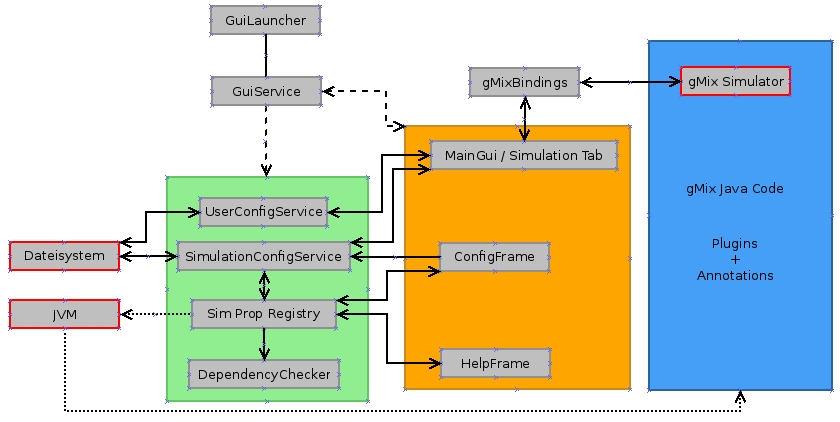
\includegraphics[width=\textwidth]{img/arch.png}
\caption{Aufrufhierarchie}
\label{fig:callgraph}
\end{figure}

% subsubsection uebersicht (end)

\subsection{Wichtige Komponenten} % (fold)
\label{ssub:einzelne_komponenten}
In diesem Unterabschnitt werden die wichtigsten Komponenten der \emph{gMix-Simulator-GUI} behandelt, welche teilweise in Abbildung \ref{fig:callgraph} schon dargestellt wurden.

\subsubsection{SimPropRegistry}
\label{sssub:simpropregistry}
Die Klasse \emph{SimPropRegistry} ist die wohl wichtigste (und auch komplexeste) Hauptkomponente der gMix-Simulator-GUI. Ihre Aufgabe besteht darin, den gesamten Code des gMix-Simulators nach Annotationen abzusuchen und die in den Annotationen enthaltenen Informationen zu verarbeiten. Die \emph{SimPropRegistry} kennt dabei drei unterschiedliche Typen von Annotationen.

\begin{enumerate}
	\item Property Annotations (aka. SimProp)
	\item Plugin Annotations (aka. SimGuiPlugin)
	\item PluginSuperclass Annotations (aka. SimGuiPluginSuperclass)
\end{enumerate}

Die einzelnen Annotation-Typen wurden bereits in Abschnitt \ref{sub:annotations} erläutert. Die \emph{SimPropRegistry} erzeugt anhand dieser Annotations dann Plugin- und Property-Objekte, welche zur Laufzeit in verschiedenen Maps verwaltet werden. Neben den beiden wichtigsten Maps (\emph{properties} und \emph{plugins}), werden noch weitere Maps gehalten, welche beispielsweise die Menge der aktuell in der GUI ausgewählten Plugins halten (\emph{activePlugins}) oder aber andere zur Laufzeit wichtige Informationen speichern.\\

Des weiteren bietet die \emph{SimPropRegistry} einige Methoden an, um auf die Inhalte eben dieser Maps zuzugreifen. So beispielsweise eine Methode (\emph{setValue}), um Werte einer vorhandenen Property zu ändern. Die Plugin-Objekte hingegen sind komplett unveränderlich, da sie keine Informationen halten, die vom Benutzer editierbar sind. Es gibt allerdings die Methode (\emph{setActivePlugins}. Mit ihr kann die Auswahl der aktiven Plugins festgelegt werden. Die Information darüber welche Plugins aktiv sind, muss der \emph{SimPropRegistry} bekannt sein, da dieses beim Schreiben der Konfiguration wichtig ist. Wir haben uns entschieden diese Informationen direkt in der \emph{SimPropRegistry} zu halten. Bei einer Zustandsänderung bezüglich der Konfiguration wird dann die \emph{SimPropRegistry} informiert und kann reagieren. Alternativ wäre es auch möglich gewesen, dass die \emph{SimPropRegistry} an kritischen Stellen das entsprechende GUI-Element nach seinem aktuellen Zustand fragt, dieses würde jedoch eine höhere Kopplung bedeuten, da die \emph{SimPropRegistry} dann die relevanten GUI-Elemente kennen müsste, weswegen wir diesen Weg vermieden haben.\\

Die \emph{SimPropRegistry} selbst ist als Singleton implementiert. Der Zugriff auf die \emph{SimPropRegistry} erfolgt über eine statische Methode (\emph{getInstance}) und kann an jeder Stelle im Code durchgeführt werden --- Diese Entscheidung wurde getroffen, da dieser Dienst in sehr vielen Komponenten der GUI verwendet wird und ein Durchreichen der Referenz in alle Komponenten sehr aufwändig und unübersichtlich wäre. 

\subsubsection{SimProp} % (fold)
\label{ssub:simprop}
Die Klasse \emph{SimProp} ist eine abstrakte Klasse und bildet die Oberklasse für die fünf typabhängigen Unterklassen (siehe Abb. \ref{fig:field_annotation}), die es zur Laufzeit geben kann. Die Felder der SimProp Unterklassen wurden bereits in  \\

\begin{figure}[!htp]
\begin{tikzpicture}
\umlsimpleclass[fill=blue!10]{SimProp}
\umlemptyclass[x=-3.5, y=-2, fill=blue!10]{BoolProp}
\umlemptyclass[x=-1.2, y=-2, fill=blue!10]{IntProp}
\umlemptyclass[x=1.2, y=-2, fill=blue!10]{FloatProp}
\umlemptyclass[x=3.9, y=-2, fill=blue!10]{DoubleProp}
\umlemptyclass[x=6.7, y=-2, fill=blue!10]{StringProp}
\umlVHVinherit[arm2=-1.2cm]{BoolProp}{SimProp}
\umlVHVinherit[arm2=-1.2cm]{IntProp}{SimProp}
\umlVHVinherit[arm2=-1.2cm]{FloatProp}{SimProp}
\umlVHVinherit[arm2=-1.2cm]{DoubleProp}{SimProp}
\umlVHVinherit[arm2=-1.2cm]{StringProp}{SimProp}
\end{tikzpicture}
\caption{Vererbung der Property Annotations}
\label{fig:field_annotation}
\end{figure}

 Obwohl alle Typen sehr viele Gemeinsamkeiten aufweisen, ist eine Typunterscheidung notwendig, da je nach Typ sich die Annotations ein klein wenig unterscheiden (siehe \ref{ssub:feld_annotation}). So ergibt es beispielsweise keinen Sinn, einem \emph{boolean} oder \emph{String} einen Minimal- oder Maximalwert zuweisen zu wollen, während dieses bei \emph{int}, \emph{float} und \emph{double} durchaus sinnvoll erscheint. Ein weiterer Vorteil ist, dass die Typkonversion und die Prüfung auf gültige Eingaben (sowie die Fehlerbehandlung) auch in die Unterklassen ausgelagert werden können, was der Lesbarkeit des Codes sehr dienlich ist. 

\subsubsection{UserConfigService} % (fold)
\label{ssub:userconfigservice}
Der UserConfigService verwaltet die user.properties. In dieser Datei werden benutzerspezifische Einstellungen abgespeichert. Der Zugriff auf diese Datei ist nur aus dieser Klasse möglich. Beispiele für benutzerspezische Einstellungen sind z.B. die größe der einzelnen Fenster und ob sie separiert dargestellt werden.

\subsubsection{Requirement} % (fold)
\label{ssub:requirement}
Um die Abhängigkeiten zwischen verschiedenen Propertys darzustellen werden Requirements (Anforderungen) verwendet. Eine Anforderung wird dabei immer speziell für eine Property geschrieben. Um dem Entwickler maximale Freiheit zu gewähren kann die Abhängigkeit beliebig komplex gewählt werden.
Generell wird zwischen zwei Anforderungen unterschieden:
\begin{enumerate}
	\item Enable Requirements: Anforderungen die dazu führen das bestimmte Propertys in Abhängigkeit zu anderen Property und deren Werten aktiviert oder deaktiviert werden.
	\\Ein Beispiel hierfür ist das "`Simulation Time End"' Requirement. Die Simulation kann entweder durch "`Real Time"' beendet werden oder durch "`Simulation Time"'. Die beiden Optionen schließen sich somit gegenseitig aus. Daher ist es hier sinnvoll sie entsprechend zu deaktivieren/ aktivieren um den Benutzer zu unterstützen.
	\item Value Requirements: Anforderungen die dazu führen das bestimmte Propertys in ihrem Wertebereich eingeschränkt werden. Dabei wurde die Implementation so gewählt, dass der vom Plugin Entwickler gewählte Wertebereich nicht erweitert werden kann weil dieses zu nicht sinnvollen Ergebnissen im Simulator führen würde.
	\\ Ein Beispiel für ein Value Requirement ist die Einschränkung aufgrund von Minimal und Maximalwerten. Wenn eine Abhängigkeit zwischen diesen festgelegt wurden gilt u.a. das aktuelle Maximalwert nicht kleiner sein darf als der aktuelle Minimalwert.
\end{enumerate}

\subsubsection{DependencyChecker}
\label{sssub:dependencychecker}
Der Dependency Checker dient der Überprüfung von verschiedenen Abhängigkeiten von einzelnen in den SimProperties definierten Anforderungen (Requirements).
Der Check findet bei jeder Änderung in der GUI statt. Im Fehlerfall, also wenn eine Anforderungen nicht eingehalten wird, gibt es zwei Fehlermechanismen:
\begin{enumerate}
	\item Enable Requirements: Die momentan nicht mögliche Simproperty wird deaktiviert. Somit ist ein Auswählen / ändern nicht mehr möglich.

\begin{figure}[!htp]
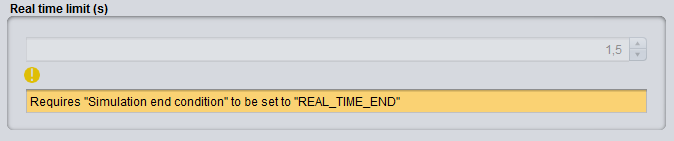
\includegraphics[width=\textwidth,scale=0.5]{img/DependencyChecker_RealTimeDisabled}
\caption{Deaktivierte Real Time End Property}
\label{fig:deactivatedRealTimeEnd}
\end{figure}

	\item Value Requirements: Falls neu gesetzte Werte aufgrund von Abhängigkeiten nicht mehr möglich sind werden individuelle, in den Value Requirements definierte, Fehlermeldungen direkt in der Simpropery angezeigt.
	
	\begin{figure}[!htp]
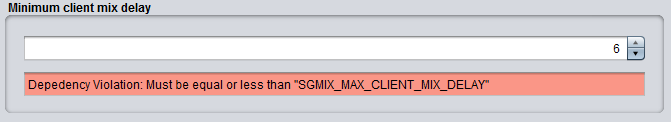
\includegraphics[width=\textwidth,scale=0.5]{img/DependencyChecker_MiniumClientMixDelayError}
\caption{Fehlermeldung bei Verstoß gegen Value Anforderungen}
\label{fig:errorMessageValueRequirement}
\end{figure}
\end{enumerate}

% subsubsection accordion (end)

\subsubsection{gMixBinding} % (fold)
\label{ssub:gmixbinding}
Die Klasse \emph{gMixBinding} ist eine Helfer-Klasse, die von der GUI verwendet wird, um dem \emph{gMix-Simulator} mit der Konfiguration aus der GUI aufzurufen. Dazu war es notwendig, den Konstruktor des \emph{gMix-Simulators} so zu erweitern, dass er die Konfiguration als \emph{passthroughParameters} entgegennimmt. Der Aufruf des Simulators erfolgt als neuer Thread. Damit blockiert die GUI nicht, während die Simulation durchgeführt wird. Nachdem der Aufruf des \emph{gMix-Simulators} zurückkehrt, wird der Pfad zum Plot an eine Factory weitergereicht, welche ein GUI-Element (\emph{}) erstellt, das für die Darstellung der Ergebnisse verantwortlich ist.\\

Ein bislang ungenutztes Feature, welches aber berücksichtigt wurde ist, dass in dem \emph{gMixBinding} das \emph{ResultSet} bereitgestellt wird des Simulators. Dieses beinhaltet die während der Simulation aufgezeichneten Statistik und kann dazu verwendet werden Ergebnisse in einer anderen Weise zu plotten, als es in der Konfiguration steht --- dieses Feature ist allerdings noch Zukunftsmusik.\\

\subsection{GUI-Elemente}
Die GUI für den gMix-Simulator wurde wie alle zuvor beschriebenen Elemente mit Java realisiert. Dies garantiert Plattformunabhängigkeit und gleiches Look and Feel auf verschiedenen Systemen. Java bietet drei unterschiedliche Layout Manager an, mit denen sich GUIs realisieren lassen.
\begin{enumerate}
\item JavaFX
\item SWT
\item Swing
\end{enumerate}
Unsere Wahl ist auf Swing gefallen, da dies ein sehr dynamisches Framework zur Erstellung einer GUI ist. JavaFX wurde hauptsächlich für den Einsatz in Webanwendungen entworfen. SWT bietet die Möglichkeiten statische GUIs zu bauen, was man beispielsweise von Produkten wie  Eclipse kennt.\\

Swing ist in der Anordnung von GUI lemente wie Buttons oder Textfeldern sehr frei und nimmt dem ntwickler große Teile des Layoutings ab. In Swing selbst werden sog. \emph{JPanel} erzeugt, in denen die GUI Elemente angeordnet werden. Die \emph{JPanel} an sich wiederrum können Bestandteil eines \emph{JFrame} sein, welches ein einfaches Fenster ist. Im Folgenden werden zwei \emph{LayoutManager} von Swing erläutert um einen Einblick in die Designmöglichkeiten des Frameworks zu geben.

\subsubsection{BorderLayout}
Das \emph{BorderLayout} ist einer der simpelsten \emph{LayoutManager} von Java Swing. Er unterteilt ein \emph{JPanel} in Fig. \ref{fig:borderlayout} gezeigten Bereiche
\begin{itemize}
    \item {PAGE\_START}
    \item {PAGE\_END}
    \item {LINE\_START}
    \item {LINE\_END}
    \item {CENTER}
\end{itemize}
welche anschließend mit Swing Komponenten befüllt werden können. Dabei ist zu bemerken, dass es sich bei den Swing Elementen wiederrum um \emph{JPanel} handeln kann, die wiederrum ihren eigenen \emph{LayoutManager} besitzen. Diese Methode ist jedoh relativ statisch und nur für das Design eines Hauptfensters zu benutzen.

\begin{figure}[!htp]
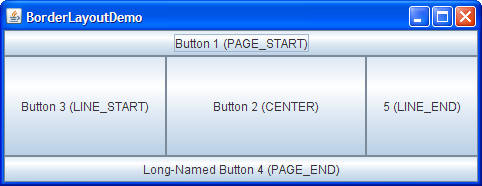
\includegraphics[width=\textwidth]{img/BorderLayoutDemo}
\caption{BorderLayout}
\label{fig:borderlayout}
\end{figure}

\subsubsection{MigLayout}
Das \emph{MigLayout} ist eine OpenSource Entwicklung, die gerade für große GUI Projekte eine besondere Agilität mit sich bringt. Bei der Verwendung des \emph{MigLayout} werden ähnlich des \emph{GridLayout} Koordinaten für einzelne GUI Elemente angegeben. Verbildlicht bedeutet dies, dass die GUI in ein Raster unterteilt wird. In dieses Raster werden die Elemente angeordnet und mit sog. \emph{Contstraints} versehen. Die \emph{Constraints} garantieren, dass die Elemente den zur Verfügung stehenden Platz nutzen, sich ordentlich orientieren oder sich in einer bestimmten Reihenfolge anordnen. Eine Auswahl von Constraints und deren Bedeutung ist unten aufgelistet:

\begin{itemize}
\item \textbf{grow} gibt an, dass ein Element den zur Verfügung stehenden Platz ausnutzen soll. Wird das Fenster vergrößert entsteht mehr Platz, der von dem Element eingenommen wird. Buttons oder Textfelder vergrößern sich somit automatisch.
\item \textbf{span} gibt an, dass ein Element sich über eine bestimmte Anzahl an Zellen ausbreiten darf. Somit lassen sich Elemente z.B. doppelt so groß wie andere Elemente zeichnen.
\item \textbf{align} gibt an, wie sich das zu zeichnende Element ausrichten soll. Klassischerweise stehen die \emph{Constraints center, left, right, top} und \emph{bottom} zur Verfügung. 
\end{itemize}

Einige nützliche Standard-Features von Swing wurden ebenso in diesem Projekt verwendet. Dazu gehören Menüs und Shortcuts. Über die Menüs, welhe am oberen Rand der Anwendung zu finden sind, lassen sich generelle Einstellungen vornehmen. Dazu zählt beispielsweise das auskoppen von einzelnen Elementen der GUI (siehe \ref{ssub:configview}, \ref{ssub:resultview} und \ref{ssub:helpview}). Die Shortcuts erlauben es dem Nutzer die komplette GUI mit der Tastatur zu bedienen. \\
Abbildungen \ref{fig:gui1} und \ref{fig:gui2} zeigen die fertige GUI des gMix Simulators. Abbildung \ref{fig:gui1} zeigt \emph{Configuration View, Simulation View, Konsole} und \emph{Results View}. In Abbildung \ref{fig:gui2} ist zusätzlich noch der \emph{Help View} zu sehen. Im WEiteren werden die einzelnen Bestandteile der GUI erläutert.

\begin{figure}[!htp]
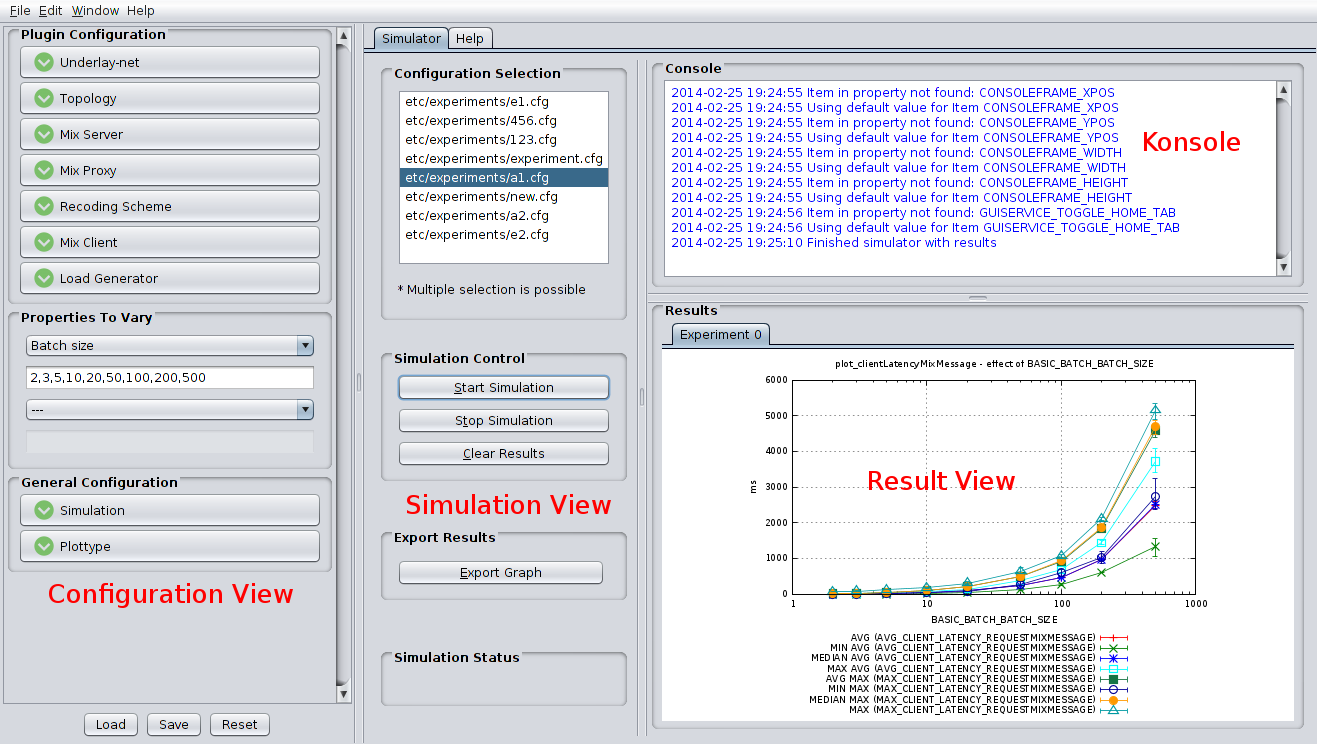
\includegraphics[width=\textwidth]{img/gmixGuiSimulator}
\caption{gMix GUI I}
\label{fig:gui1}
\end{figure}

\begin{figure}[!htp]
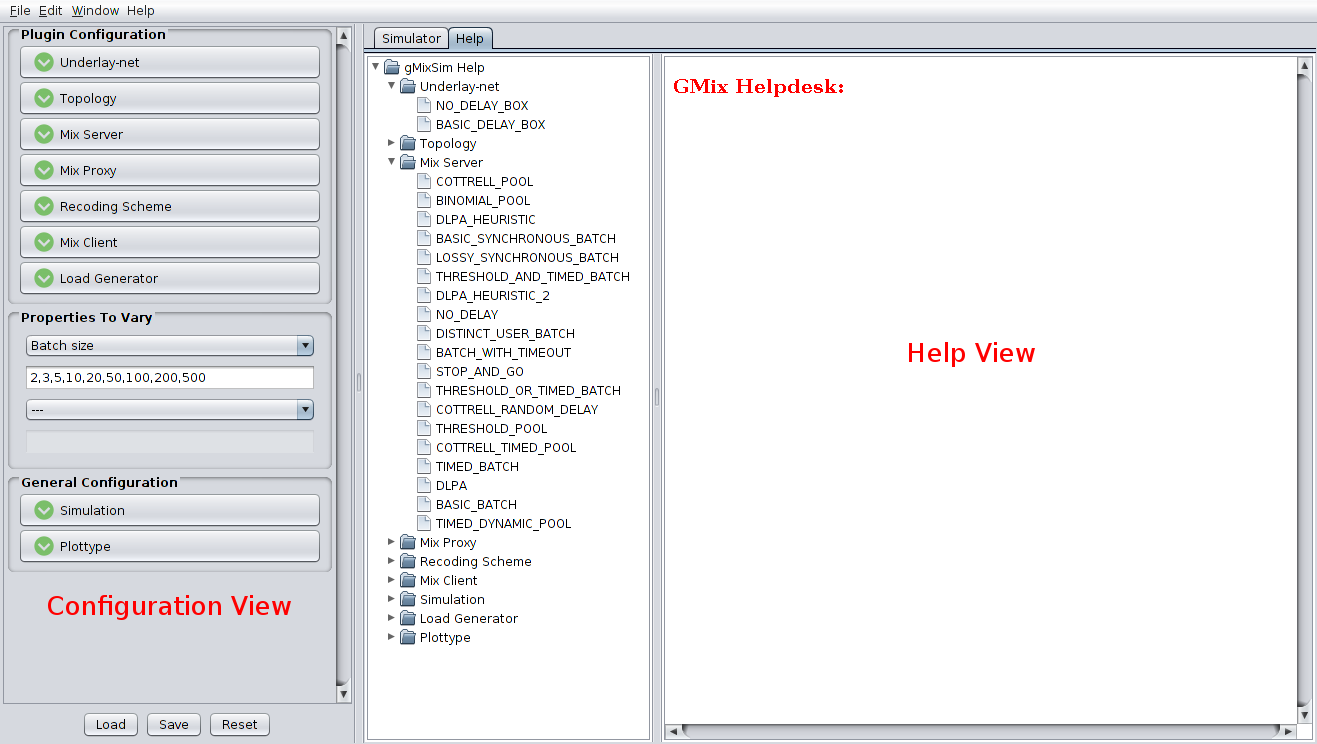
\includegraphics[width=\textwidth]{img/gMixGuiHelp}
\caption{gMix GUI II}
\label{fig:gui2}
\end{figure}

\subsubsection{Configuration View} % (fold)
\label{ssub:configview}
Der \emph{Configuration View} bildet das zusammen mit der \emph{SimPropRegistry} (vgl. \ref{sssub:simpropregistry}) das Herzstück der GUI. Mit ihr hat der Nutzer die Möglichkeit die Simulation auf einfach Art und Weise zu konfigurieren. \\
Der \emph{ConfigurationView} besteht aus den sog. \emph{AccordionEntries}, der \emph{PropertiesToVary} Konfiguration, einer allgemeinen Simulationskonfiguration und den Buttons \emph{Load, Save} und \emph{Reset}. Angelehnt an moderne Smartphone Betriebssysteme wurden die \emph{AccordionEntries} entwickelt, welche sich durch einen Button und darunter verborgene Konfigurationsmöglichkeiten auszeichnen. Jeder Layer der Simulatorkonfiguration lässt sich somit auf einen Button abbilden unter dem ein Plugin für diesen gewählt werden kann. In der vorliegenden Version der gMix-Simulator GUI werden folgende Layer verwendet:
\begin{enumerate}
\item \textbf{Underlay-net}, dass zugrundeliegende Netzwerk
\item \textbf{Topology}, dessen Aufbau
\item \textbf{Mix Server}, das Verhalten des Mix Servers
\item \textbf{Mix Proxy}, die Proxykonfiguration
\item \textbf{Recoding Scheme}, die Art der Umkodierung
\item \textbf{Mix Client}, der Client
\item \textbf{Load Generator}, die Verkehrsdatenerzeugung
\end{enumerate}
 Klickt man auf den Button erhält man zunächst eine Auswahl in Form einer Combobox um ein Plugin zu wählen. Hat man in Plugin gewählt erhält man die Konfigurationsmöglichkeiten für dieses Plugin. Dabei wird die Anzeige dynamisch, ausgehend vom Variablentyp der \emph{SimulationProperty} erstellt. Der Typ wurde zuvor vom Entwikler per \emph{Annotation} festgelegt. Zwei Beispiele für dynamisch erzeugte Konfigurationsmöglichkeiten sind
 \begin{itemize}
 \item \textbf{Integer} wird über einen Spinner konfiguriert. 
 \item \textbf{Boolean} wird mit einer Checkbox konfiguriert.
 \end{itemize}
 Diese Konfiguration ermöglicht es dem Nutzer sofort die Übersicht über seine Konfigurationsmöglichkeiten zu erhalten. Zusätzlih werden Fehlkonfigurationen ausgeschlossen, da die Konfiguration auf deren Variablentypen eingeschränkt ist. Falsche WErteingaben werden mit Hilfe des Dependency Checkers (vgl. \ref{sssub:dependencychecker}) verhindert. \\
 Unter der Pluginkonfiguration befindet sich die Konfiguration für die \emph{PropertiesToVary}. Diese geben an, welche Properties bei der Simulation variiert werden sollen. Die Eingabe wird hier über eine simple Textbox realisiert um die Koniguration möglichst offen zu gestalten. \\
 Den letzten Abschnitt im \emph{Configuration View} bilden die allgemeinen Einstellungen zur Simulation und dem Plottype. Diese wurden ebenfalls als \emph{AccordionEntry} dargestellt um die Übersichtlichkeit zu bewahren. Der Eintrag Simulation bietet beispielsweise die Option den Endzeitpunkt einer Simulation zu konfigurieren. Unter dem \emph{AccordionEntry} Plottype lässt sich unter anderem das Plotskript für Gnuplot definieren.\\
 Nach der Konfiguration einer Simulation kann diese über den Button \emph{Save} abgespeichert werden. Dabei werden alle Einstellungen in ein einheitliches Konfigurationsdateiformat gespeichert. Die so generierten Konfigurationsdateien lassen sich einfach wiederverwenden und sind zusätzlich übersichtlich gestaltet. Über den Button \emph{Load} lässt sich eine so zuvor gespeicherte Konfigurationsdatei wieder öffnen und in den \emph{Configuration View} laden. Dabei werden alle \emph{Accordion Entries} aufgeklappt um eine direkte Übersicht über die Konfiguration zu ermöglichen. Der Button \emph{Reset} setzt die Einstellugen auf eine Standardkonfiguration zurück. Möchte man eine definierte Konfiguration ausführen muss diese zuvor gespeichert werden um im Simulation View (in Abschnitt \ref{ssub:simulationview} erläutert) auswählbar zu sein.\\
 Nach der Konfiguration einer Simulation kann diese über den Button \emph{Save} abgespeichert werden. Dabei werden alle Einstellungen in ein einheitliches Konfigurationsdateiformat gespeichert. Die so generierten Konfigurationsdateien lassen sich einfach wiederverwenden und sind zusätzlich übersichtlich gestaltet. Über den Button \emph{Load} lässt sich eine so zuvor gespeicherte Konfigurationsdatei wieder öffnen und in den \emph{Configuration View} laden. Dabei werden alle \emph{AccordionEntries} aufgeklappt um eine direkte Übersicht über die Konfiguration zu ermöglichen. Der Button \emph{Reset} setzt die Einstellugen auf eine Standardkonfiguration zurück. Möchte man eine definierte Konfiguration ausführen muss diese zuvor gespeichert werden um im Simulation View (in Abschnitt \ref{ssub:simulationview} erläutert) auswählbar zu sein.\\
 Zur Unterstützung der Übersichtlichkeit bietet die GUI die Möglichkeit den \emph{Configuration View} vom Hauptfenster auszukoppeln. ies ist besonders hilfreich wenn man z.B. mit mehreren Monitoren abeitet oder das Hauptfenster ohne die Konfiguration betrachten möchte. Dabei wird ein neues Fenster erzeugt, welches nur den \emph{Configuration View} enthält.

\subsubsection{Simulation View} % (fold)
\label{ssub:simulationview}
Der \emph{Simulation View} lässt den Nutzer seine vorher gespeicherte Konfiguration ausführen und generiert direkt einen Graphen mittels Gnuplot. Dadurch sind die Ergbnisse der Simulation sofort einzusehen. Der \emph{Simulation View} besteht aus drei Komponenten. AUf der linken Seite sind die vorhandenen Konfigurationsdateien zu sehen. Diese können per Multiselect (d.h. mehrere auf einmal) in der \emph{Configuration Selection} ausgewählt werden. Mit Hilfe der \emph{Simulation Control} kann die Simulation gestartet (\emph{Start Simulation}) oder angehalten (\emph{Stop Simulation}) werden. Die generierten Ergebnisse können mittels \emph{Clear Results} gelöscht werden. Zur Laufzeit des Programms werden die generierten Dateien jedoch nicht gelöscht, sondern nur aus der Anzeige entfernt. Über \emph{Export Results} lassen sich generierte Graphen in zwei verschiedene Formate expertieren. Zur Verfügung stehen .png und .eps. Beim Start einer Simulation erscheint im \emph{Simulation Status} ein Fortschrittsbalken, der signalisiert, dass die Simulation im Gange ist. \\
Auf der rechten Seite des \emph{Simulation View} befindet sich in der oberen Hälfte die Konsole (siehe \ref{ssub:consoleview}). Darunter ist der \emph{Result View} (siehe \ref{ssub:resultview}) angesiedelt.

\subsubsection{Result View} % (fold)
\label{ssub:resultview}
Der \emph{Result View} präsentiert die Ergebnisse der zuvor ausgewählten Simulation. In der vorliegenden Version der gMix Simulator GUI wird Gnuplot zum rendern der Ergebnisse verwendet. Nach erfolgreicher Simulation wird im \emph{Result View} ein Tab erzeugt, der den dazugehörigen Graphen anzeigt. Ergebnisse werden in der Reihenfolge generiert, wie sie von oben nach unten in der Liste der \emph{Configuration Selection} ausgewählt wurden. Zusätzlich gibt die Legende der Graphen Auskunft um welche Simulation es sich handelt. Die Ergebnisse werden mittels des zuvor definierten Plotskripts erstellt. Gnuplot liefert das Ergebnis als Vektorgrafik, damit diese in der GUI ordentlich skaliert. Über die in \ref{ssub:simulationview} beschriebene Funktion lässt sich der Graph auch in andere Formate exportieren und speichern. Löschen lassen sich erstellte Ergebnisse mit Hilfe des Buttons \emph{Clear Results}. Um die Ergebnisse vergrößert zu betrachten genügt ein Rechtsklick auf das Ergebnis um über das Menü den Graphen von der GUI zu entkoppeln. So können mehrere Ergebnisse gleichzeitig vergrößert, entkoppelt und gegeneinander gestellt werden. 

\subsubsection{Konsole} % (fold)
\label{ssub:consoleview}
Die \emph{Konsole} der gMix Simulator GUI gibt Auskunft über den aktuellen Status der GUI und den Fortschritt der Simulation. Speziell für diese Zwecke wurde der Logger \emph{log4j} von Apache um einen Appender erweitert, welcher bei einem bestimmten Loglevel in die \emph{Konsole} schreibt. Somit lassen sich die Nachrichten auf der \emph{Konsole} von Nachrichten, die in logs gespeichert werden unterscheiden.

\subsubsection{Help View} % (fold)
\label{ssub:helpview}
Der \emph{Help View} bietet dem Anwender Unterstützung bei der Benutzung der GUI. Ausgehend von den registrierten Plugins wird die Hilfe angelehnt an die Anordnung der \emph{Accordion Entries} aufgebaut. Dabei entsteht eine Baumstruktur, die mittels \emph{JTree} umgesetzt wurde. Als Blätter des \emph{JTree} werden die verfügbaren Plugins aufgezeigt. Wählt man ein Element aus öffnet die GUI eine HTML-Datei, welche zuvor vom Pluginentwickler angelegt wurde. Dabei ist zu beachten, dass die HTML-Datei den gleichen Namen wie der Plugin-Key hat. Somit werden Kollisionen vermieden und eine eindeutige Zuordnung von Plugin zu Hilfe erstellt. Der \emph{Help View} lässt sich wie der \emph{Configuration View} auskoppeln um das gleichzeitige Arbeiten an der Simulation und Nachschlagen in der Hilfe zu erleichtern.

\subsubsection{Bedienungsablauf in der GUI}
\label{ssub:bedienung}
In der Reihenfolge der zuvor aufgezählten GUI Elemente lässt sich einfach eine Simulation durchführen. Für den schnellen Einstieg folgt  ein HowTo:

\begin{enumerate}
\item \textbf{Auswahl der Plugins:} \newline Der Benutzer wählt im \emph{Configuration View} die gewünschten Plugins mit Hilfe der \emph{Accordion Entries} aus und konfiguriert diese.
\item \textbf{Auswahl der Properties To Vary:} \newline Anschließend werden die zu variierenden Werte angegeben.
\item \textbf{Simulationskonfiguration:} \newline In der \emph{General Configuration} werden Angaben zu Ende der Simulation und Plotskript gemacht.
\item \textbf{Speichern der Konfiguration:} \newline Über den Button \emph{Save} wird die vorgenommene Konfiguration gespeichert.
\item \textbf{Auswahl der zu simulierenden Konfiguration:} \newline Die soeben gespeicherte Konfiguration wird in der \emph{Configuration Selection} ausgewählt. Dank Multiselection können auch mehrere Konfigurationen gleichzeitig gewählt werden.
\item \textbf{Start der Simulation:} \newline Durch Druck auf den Button \emph{Start Simulation} wird die Simulation gestartet und anschließend werden die Ergebnisse im \emph{Results View} ausgegeben. 
\end{enumerate}
\section{Entwickler Informationen} % (fold)
\label{sec:entwicklung}

% TEST \cite{dummy:svs}.
% section features (end)

% \bibliographystyle{plain}
% \bibliography{references}

%----------------------------------------------------------------------------------------

\end{document}